\chapter{Approach}
\label{chapter:approach}



\chapter{Key Concepts}
Our approach aims to help software developers in remote teams who might be facing challenges with workplace isolation, team awareness, informal communication within their team, and well-being. We aim to tackle these issues by allowing knowledge workers to easily learn about the availability, moods and emotions, and other states of their core team members. The key underlying concepts of our approach listed and explained in the following.

\medskip\noindent\textbf{Ambient always-on-top, people-centered team view} \\
At the core of our approach sits the desicion to create a tool that is ambient in nature and does not require significant, additional effort in order to be useful. Having a limited amount of information on an ambient display is critial for both not being interruptive and costly to use \autocite{dabbish2004controlling}. With the help of the ambient display, the goal is to create a sense of presence within the team, even when working from different locations. By constantly showing the most important team members the goal is to minimize the feeling of being left and to foster a sense of belonging.

In comparison to existing awareness inceasing approaches with emphasis primarily on task related awareness and their implications for more effective and efficient collaboration, our approach puts the humans behind the work items into the center of focus. By fostering a more social communication, our approach does not conflict with or replace existing communication patterns that are established in a company. Rather, it should be looked at additional, social information about the individual team members.

\medskip\noindent\textbf{Transience and topicality} \\
We want to keep interactions very "light-weight" and casual, which is why the functionality is very simple, maybe even limited, by design. The information shared and displayed will be of transient nature. Following this approach brings the benefit of really fostering informal communication because there is no guarantee that messages will be read. In addition, our approach visually emphasises on the topciality of information displayed in order to avoid outdated data that clutters the user interface.

\medskip\noindent\textbf{Mood and context sharing} \\
As the main text-based informal communication possibility, our approach focuses on status messages to can be broadcasted to the entire team. This conecept is also known as micro-blogging, with the difference that common micro-blogging platform often times are public (e.g. twitter) and our approach is scoped to a team. \textcite{dullemond2013fixing} state that micro-blogging is another strategy that allowed software engineers to share activities and moods with other team members with the result of feeling more connected to each other. Our approach is very similar to theirs in terms of functionality of the mood-based status sharing, yet we do not force the users to always share moods together with a status message; we are interested in use cases for the combined and isolated usage of the two features. Further, topics that are usually blogged about are informal \autocite{ehrlich2010microblogging} which aligns with the goal of our approach. Furthermore, mood sharing seems to acts as a springboard for conversations according to \textcite{church2010study}.

\medskip\noindent\textbf{Ever-running break room} \\
Additionally, allowing to actually see the team (and not just relying on text-based information), is possible by joining an ever-running break room. The goal is to mimick the water-cooler in the office. Thus, visiting a breakroom as simple as possible, similar to just walking to the coffee machine in an office and signaling to the other team members that you are now on a break is a requirement. This is motivated by \textcite{chang2007out}, which emphasize that initiating a conversation must be as simple as possible. This approach also applies to the next concept on the list, interactions that target individual team members.

\medskip\noindent\textbf{1:1 interactions} \\
For scenarios where the content you want to share isn't intended for a single person, or you simply want to get another team member's attention, there's an easy way to start a private conversation. This can be done through a direct message or by nudging a team member. This concept aims to help in cases of help seeking, a known problem when working remotely \autocite{herbsleb2003empirical}. Recalling the transient nature of our approach, this communication mechanism is best suited for making a non-interruptive request that is not urgent. Should a user feel the need of talking to another team member, he/she has the possibility to indicate that now would be an appropriate time for a short informal communication. If other team members feel the same, random matches can be made and the two team members join a virtual video call.

\medskip\noindent\textbf{Minimizing interruptions} \\
When developing an ambient always-on top visualization, minimizing interruptions and distractions is one of the most important design principles. Specifically, this means a very targeted use of notifications and the ability to not be contacted and hide potential distractions if desired.

\chapter{Prototype}
The above outlined key concepts were then developed into the key features of our research prototype, \textit{AmbientTeams}. Before stepping in to the core features employed in AmbientTeams and aligning them to the above mentioned key concepts, a brief introduction into the more technical aspects and a general overview of the application is given.

AmbientTeams is a cross-platform desktop application based on Electron\footnote{\url{https://www.electronjs.org/}}. To facilitate the implementation of the interactive user interface, VueJS\footnote{\url{https://vuejs.org/}} was used. To maintain JavaScript as a common language for the front-end and back-end, NodeJS\footnote{\url{https://nodejs.org/}} is used on the server side. The server provides both a REST API for basic CRUD functionality for users and teams, as well as a websocket endpoint, since much of the data required for AmbientTeams comes from the server in real time.

AmbientTeams comes with two main windows. The overview window is responsible for maintaining a connection to the server, authenticating, login functionality, settings. Additionally, once the user has authenticated, he/she is redirected to the overview view where all teams and team members are visible (see \autoref{fig:at_overview}). By clicking on the edit icon next to the team name, the user has the possibility to pick a selection of team members from each team that will then be displayed on the other main window, the ambient window. This is demonstrated in the team called "AmbientTeams" in \autoref{fig:at_overview}.

\begin{figure}[h]
    \centering
    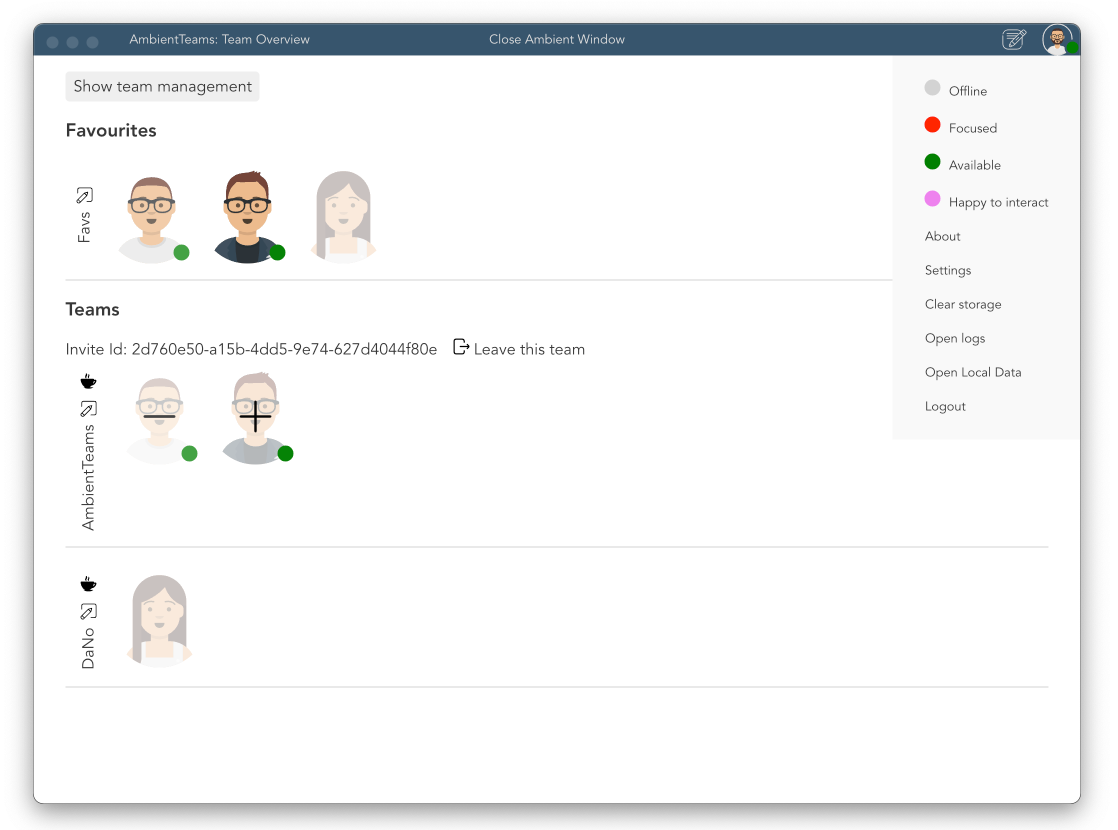
\includegraphics[width=.8\linewidth]{./images/AT_overview.png}
    \caption{Overview Window }
    \label{fig:at_overview}
\end{figure}

\medskip\noindent\textbf{Ambient always-on-top, people-centered team view} \\
AmbientTeams consists of two main windows; an overview window and the so-called ambient window. To keep the ambient overlay as ambient and minimal as possible, a transparent window was chosen. Further, certain functionality is only visible when the user is hovering over this window. When hovering, the user can select the team they want to show

\begin{figure}[h]
    \centering
    \begin{subfigure}{.5\textwidth}
        \centering
        
\includegraphics[width=.8\linewidth]{./images/AT_no_hover.png}
        \caption{No hover }
        \label{fig:at_no_hover}
    \end{subfigure}%
    \begin{subfigure}{.5\textwidth}
        \centering
        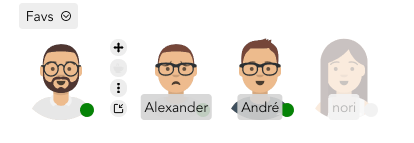
\includegraphics[width=.8\linewidth]{./images/AT_hover.png}
        \caption{Hover }
        \label{fig:at_hover}
    \end{subfigure}
    \caption{Ambient Window}
\end{figure}

\medskip\noindent\textbf{Transience and topicality} \\
\medskip\noindent\textbf{Mood and context sharing} \\
\medskip\noindent\textbf{Ever-running break room} \\
\medskip\noindent\textbf{1:1 interactions} \\
\medskip\noindent\textbf{Minimizing interruptions} \\

\chapter{Preliminary Evaluation}
To evaluate the above mentioned research questions, a small pilot study was conducted Optimising and improving our approach with the help of feedback from a small team consisting of knowledge workers is the main goal of this master thesis. Further, by collecting additional data hope to get valuable first insights into the following areas:

\begin{enumerate}
    \item Common workflows and patterns \\
          \textit{RQ1:} How do knowledge workers use and interact with AmbientTeams? How do they integrate it into existing workflows?
    \item Mood sharing behavior \\
          \textit{RQ2:} Do knowledge workers want to share their moods with their remote team members? If so, what causes knowledge workers to share their moods with their team?
    \item Feeling of isolation \\
          \textit{RQ3:} Can a people-focused team mood and status sharing approach decrease the feeling of isolation in remote knowledge worker teams?
    \item Information consumption \\
          \textit{RQ4:} What do knowledge workers learn from information shared by their team members? What kind of information is the most valuable?
\end{enumerate}

The data used to answer the above research questions came from three different sources. Given the relatively few participants, it was important to have both quantitative and qualitative data. After having a look at the study procedure in the next chapter, each of the three data sources and their relevance for the research questions are elaborated.

To find participants, a recruitement flyer (see .) The study was conducted with two knowledge worker teams, each team fulfilling the following paritication requirements:

\begin{enumerate}
    \item At least 3 team members
    \item Three or more common working days a week
    \item Spending the majority of their work day on the computer
    \item Having all the required rights to install AmbientTeams on their work computer
    \item Willingness to use AmbientTeams during at least 3 full days of work (approximately 0800 - 1700)
    \item Using macOS or Microsoft Windows
    \item An active internet connection
\end{enumerate}

\section{Procedure}
\begin{enumerate}
    \item Initial meeting: Installation, registration, team creation, give each team member a participant ID (see \autoref{subsection:initial_meeting})
    \item Pre-study questionnaire (see \autoref{subsection:questionnaires})
    \item Evaluation phase (see \autoref{subsection:evaluation})
    \item Post-study interview (see \autoref{subsection:interview}) with data collection (see \autoref{subsection:data_collection})
    \item  Post-study questionnaire (see \autoref{subsection:questionnaires})
\end{enumerate}

\section{Initial meeting}
\label{subsection:initial_meeting}
Installation

\section{Pre- and post-study Questionnaires}
\label{subsection:questionnaires}
The pre and post study questionnaires are used to asses the feeling of workplace isolation before and after the evaluation period. The questions are taken from ....

\section{Evaluation Phase}
\label{subsection:evaluation}
How long? \\
During the study notes from notion

\section{Interview}
\label{subsection:interview}
Interview questions and their relevance for the research questions

\section{Data Collection}
\label{subsection:data_collection}
\autoref{table:data_collection} shows an overview of all data collected and for which research question they are relevant.

\begin{table}[h]
    \centering
    \begin{tabular}{ |c|c|c| }
        \hline
        Data collected & Storage & Relevant for \\
        \hline
        cell4          & Local   & cell5        \\
        cell7          & Local   & cell8        \\
        \hline
    \end{tabular}
    \caption{The data collected during the preliminary evluation and its relevance for the RQs}
    \label{table:data_collection}
\end{table}